\documentclass{article}

\usepackage{tikz}
\usetikzlibrary{automata, positioning}
\begin{document}
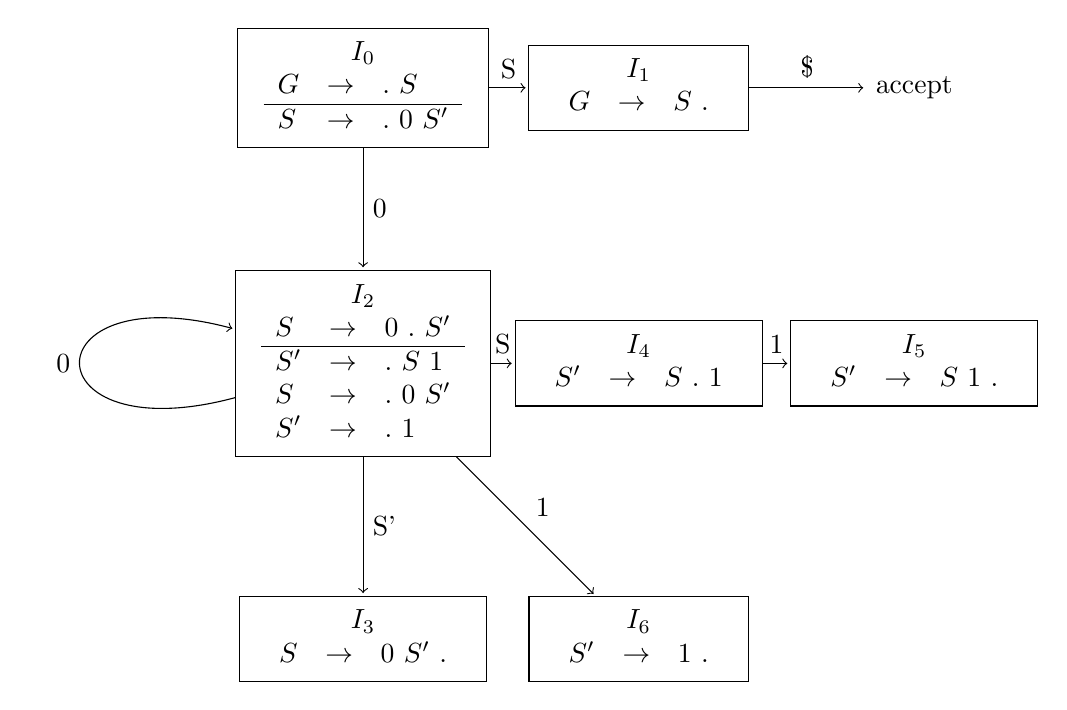
\begin{tikzpicture}[shorten >= 1pt, node distance = 3.5cm, on grid, auto]
  \node[state, rectangle] (0) {
    \begin{tabular}{c} $I_0$ \\
      $\begin{array}{lcl} 
        G &\rightarrow& .~S \\
        \hline
        S &\rightarrow& .~0~S' \\
      \end{array}$
    \end{tabular}};
  \node[state, rectangle] [right=of 0] (1) {
    \begin{tabular}{c} $I_1$ \\ 
      $\begin{array}{lcl} 
        G &\rightarrow& S~. \\
      \end{array}$
    \end{tabular}};
  \node[state, rectangle] [below=of 0] (2) {
    \begin{tabular}{c} $I_2$ \\ 
      $\begin{array}{lcl} 
        S &\rightarrow& 0~.~S' \\
        \hline
        S' &\rightarrow& .~S~1 \\
        S &\rightarrow& .~0~S' \\
        S' &\rightarrow& .~1 \\
      \end{array}$
    \end{tabular}};
  \node[state, rectangle] [below=of 2] (3) {
    \begin{tabular}{c} $I_3$ \\ 
      $\begin{array}{lcl} 
        S &\rightarrow& 0~S'~. \\
      \end{array}$
    \end{tabular}};
  \node[state, rectangle] [right=of 2] (4) {
    \begin{tabular}{c} $I_4$ \\ 
      $\begin{array}{lcl} 
        S' &\rightarrow& S~.~1 \\
      \end{array}$
    \end{tabular}};
  \node[state, rectangle] [right=of 4] (5) {
    \begin{tabular}{c} $I_5$ \\ 
      $\begin{array}{lcl} 
        S' &\rightarrow& S~1~. \\
      \end{array}$
    \end{tabular}};
  \node[state, rectangle] [below=of 4] (6) {
    \begin{tabular}{c} $I_6$ \\ 
      $\begin{array}{lcl} 
        S' &\rightarrow& 1~. \\
      \end{array}$
    \end{tabular}};
  \node[] (100) [right=of 1] {accept};
  \path[->]
    (0) edge node {S} (1)
        edge node {0} (2)
    (2) edge node {S'} (3)
        edge [loop left] node {0} (2)
        edge node {S} (4)
        edge node {1} (6)
    (4) edge node {1} (5)
    (1) edge node {\$} (100);
\end{tikzpicture}
\end{document}
